\chapter{Baggrund}
\section{Blodtryk}
Lungekredsløbet og det store kredsløb består begge af et lukket system af blodkar. Ud fra aorta udgår der arterier i det store kredsløb, der transporterer blod til organerne. \\\\
Aorta og arterierne i det store kredsløb udsættes for det højeste tryk. De mindste arterier kaldes aterioler, som forgrener sig til kapillærer. Udveksling af næringsstoffer, affaldsstoffer og luftarter mellem blodet og cellerne foregår mellem kapillærvæggen, hvilket er kredsløbets vigtigste opgave. Alle andre dele af kredsløbet sørger for, at der transporteres tilstrækkeligt blod til kapillærerne i de forskellige organer. Stofudvekslingen foregår tilstrækkeligt hurtigt, da afstanden mellem cellerne og de nærmeste kapillærer er meget lille. Kapillærerne forgrener sig til venoler, der samler sig i vener, som udmunder i hjertet. Venolerne og venerne transporterer blodet tilbage til hjertet samtidig med, at venerne er depot for blod. \\\\Væskestrømningen er det væskevolumen, der fragtes gennem et rør pr. tidsenhed. Væskestrømningen, Q, stiger med trykforskellen i begyndelsen og slutning af røret, $\Delta$P, samt aftager med rørets modstand mod væskestrømmen, R: 

\begin{equation}
\centering
Q = \frac{\Delta P}{R}
\end{equation}

Trykforskellen udgør drivkraften for væskestrømmen gennem røret. Denne strøm går fra højt til lavt tryk, hvilket hjertets kontraktion fremkalder. Modstanden i røret er et udtryk for gnidningsmodstanden mellem den væske, der bevæger sig og rørvæggen, som er i ro. Denne modstand har indflydelse på væskestrømmen i et rør. Efterhånden som væsken strømmer gennem røret, falder trykket i væsken. Ved stigende modstand mod væskestrømmen, stiger dette trykfald. Når modstand mod væskestrømmen i røret stiger, bliver væskestrømmen mindre under forudsætning af, at trykforskellen ikke stiger tilsvarende. Denne modstand bestemmes af tre faktorer: rørets længde, indre diameter og væskens viskositet. 
Modstanden stiger med øget rørlængde, reduceret diameter og øget viskositet. 
\\\\Væskestrømmen i blodkar kaldes blodstrømmen. Hjertets kontraktion sætter væsken i rørene under tryk – jo kraftigere hjertet pumper, jo større bliver trykforskellen og dermed blodstrømningen. Diameteren af blodkarret har stor betydning for modstanden mod blodstrømmen. Modstanden er mindre, og blodstrømmen er større i de store kar end i de små. Modstanden, der er mod en væskestrøm aftager med radius i fjerde potens. Dette betyder, at hvis et kars diameter fordobles, bliver modstanden hele 16 gange mindre. 
I det store kredsløb er trykket lig med forskellen mellem trykket i aorta og trykket i højre atrium. Det tryk, der er i højre atrium, er ved normale tilstande meget tæt på nul, og derved kan man betragte det gennemsnitlige tryk i aorta som trykforskellen fra nul. Det arterielle blodtryk er det tryk, der er på de store arterier, som er ligeså højt som trykket på aorta. Modstanden i hele det store kredsløb kaldes den totale perifere modstand. Formlen for sammenhængen mellem væskestrøm, tykforskel og modstand kan også overføres til det store kredsløb, hvor minutvolumen, MV, stiger med blodtrykket, BT, og aftager med den totale perifere modtand, TPM:

\begin{equation}
\centering
MV = \frac{BT}{TPM}
\end{equation}

Dette betyder, at ændringerne i det arterielle blodtryk skyldes forandringer i enten hjertets minutvolumen eller blodkarrenes mostand mod væskestrømmen.
Når blodet går fra hjertet til kapillærerne forgrener blodkarrene sig til mange små og smallere kar. Herved stiger det samlede tværsnitsareal kraftigt, og der sker automatisk en aftagning af blodets strømningshastighed. Blodets lave strømningshastighed i kapillærerne er vigtig for stofudvekslingen, der sker gennem kapillærvæggene. Ved blodets vej tilbage fra kapillærerne til hjertet stiger strømningshastigheden igen, idet det samlede tværsnitsareal aftager. \\\\
Aorta og det store kredsløbs andre arterier har tykke vægge, og deres væv er meget elastisk. Deres store diameter gør, at blodstrømmen ikke modtager ret stor modstand fra arterierne, og trykfaldet langs arterierne er ligeledes ubetydelig. Derfor er arterierne gavnlige, når transporten af blod til organerne skal være hurtig og meget lidt energikrævende.\\\\
Blodmængden som en arterie modtager og den blodmængde, der sendes videre, ændres hele tiden. Trykket i aorta og de andre arterier stiger, og de elastiske fibre i karvæggen strækkes. Dette stræk kommer af den energi, som hjertet overfører til blodet. Når hjertet er i hvileposition, og arterierne dermed kun modtager lidt blod fra hjertet, trækker arterievæggene sig sammen passivt. Dette gør, at trykket i arterierne falder, og blodet kan forsat strømme videre i karsystemet, selvom der ikke pumpes blod ud af hjertet. Hjertet overfører altså en energi til arterievæggen, som bruges til at presse blodet videre i karsystemet. \\
De hurtige trykforandringer i aorta og arterierne skyldes hjertets kontraktions- (systole) og afslapningsfase (diastole). Når blodtrykket måles, bliver det angivet med to tal, som er henholdsvis det systoliske blodtryk og det diastoliske blodtryk. Det systoliske tryk er den kraft, der opstår, når der skabes et pres på arterierne ved sammentrækning af hjertet. Det diastoliske tryk er derimod det laveste tryk, som indikerer trykket, der findes i arterierne mellem hvert hjerteslag, når hjertet er i hvileposition og fyldes med blod fra de store vener. 
Ved hvile er det gennemsnitlige tryk, middeblodtrykket, tættere på det systoliske blodtryk end det diastoliske, da diastolen er længerevarende end systolen. 
Blodtryk måles almindeligvis i enheden mmHg, som er millimeter kviksølv. Dette gøres, da blodtrykket ofte måles med kviksølvmanometer.

\section{Invasiv blodtryksmåling}
Blodtryk kan måles på forskellige måder – både invasivt og non-invasivt. I begge tilfælde bestemmes en værdi for det systoliske- og det diastoliske blodtryk. Non-invasivt kan blodtrykket måles med ultralyd eller ved den oscillometriske metode med manchet, stetoskop og kviksølvsmanometer. Derudover findes der også den automatiserede teknik, der erstatter stetoskopet med en mikrofon. \\\\
Invasive blodtryksmålinger bruges ofte til monitorering af hæmodynamiske data, og anvendes som regel hos svært syge patienter på eksempelvis intensiv afdeling, samt ved større operationer. Ved den invasive blodtryksmåling måles blodtrykket via et kateter, der lægges ind i arterien. Med denne metode får man et mere præcist og kontinuerligt billede af, hvordan hjertet arbejder. 

\begin{figure}[H]
	\centering
	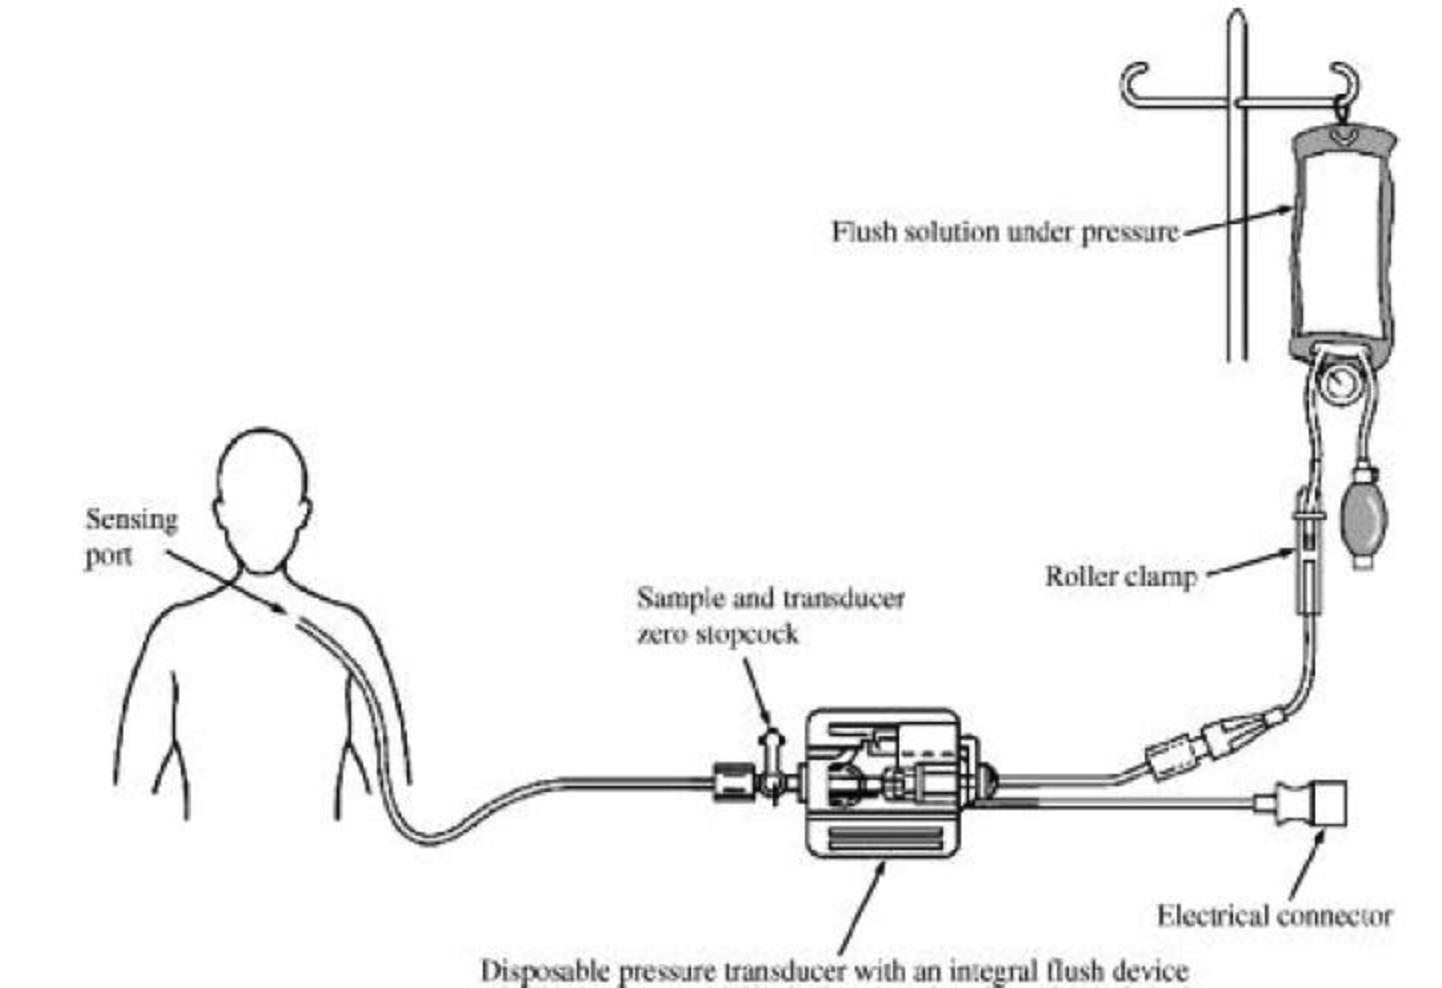
\includegraphics[width=1\textwidth]{Figurer/Snip20151207_50}
	\caption{Måleopstilling}
\end{figure}

På Figur 3.1 ses måleopstillingen for den invasive blodtryksmåling. Der føres et væskefyldt kateter ind i personens arterie. Trykposen på Figur 3.1 er fyldt med natriumklorid og fungerer som en del af flushmekanismen, som benyttes til at fjerne bobler fra det væskefyldte kateter. Trykket i posen pumpes op til mellem 180 til 300 mmHg, hvilket er over det systoliske blodtryk. \\
Slangen fra trykposen går ned til tryktransduceren og flushsystemet. Når fluchsystemet startes, vil man på monitoren kunne se, at trykket stiger til det tryk, der er i trykposen. Når dette stoppes, er systemet udviklet således, at der altid vil løbe en dråbe natriumklorid ind i kateteret. Dette forhindrer blod i at strømme ud i kateteret. Trykket i det væskefyldte kateter er lig med trykket i personens arterie. Det er dette tryk, som tryktransduceren transformerer om til et elektrisk signal, som kontinuert vises på monitoren. \\
Tryktransduceren består af fire strain gauges, også kaldet en wheatstone bro. Strain gauges er en modstandståd, der kan foldes og limes på et hvilket som helst materiale. Modstanden, R bestemmes ud fra længden, l, resistiviteten, $\varrho$ og tværsnitsarealet, A. 

\begin{equation}
	R = \frac{l \cdot \varrho}{A}
\end{equation}

Ændres en eller flere af disse, vil modstandsværdien ændres efterfølgende. Materialet, som strain gauges er limet fast på, kan ændre form, hvilket strain gauges registrerer. Det er dette, tryktransduceren benytter sig af. De fire strain gauges er limet fast på en membran, som sidder for enden af det væskefyldte kateter. Når blodtrykket ændrer sig, påvirkes membranen, da den har en meget højere compliance end selve det væskefyldte kateter. Denne forskel i compliance er en af grundene til, at dette system kan registre selv de mindste trykændringer. \\ 
Trykændringer registreres af de fire strain gauges, som transformerer dem om til det elektriske signal, hvilket afbildes grafisk. På figur 3.2 ses afbildningen af en invasiv blodtryksmåling, hvor det også er muligt at aflæse det diastoliske og systoliske blodtryk.  Det diastoliske tryk svarer til minimumspunkterne, hvor toppunkterne svarer til det systoliske tryk.


\begin{figure}[H]
	\centering
	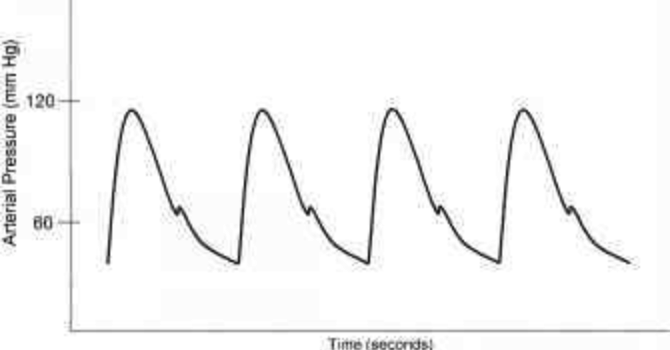
\includegraphics[width=1\textwidth]{Figurer/Snip20151207_51}
	\caption{Grafisk afbildning af en invasiv blodtryksmåling}
\end{figure}

Strain gauges benyttes i dette tilfælde, da man ønsker, at selv den mindste trykændring skal kunne registreres. Da disse modstandsændringer er så små, ønskes disse forstærkes op. For at kunne gøre dette bedst muligt, skal der benyttes et måle setup, som er centraliseret omkring nul. Til dette bruges en Wheatstone bro, nærmere en helbro, se Figur 3.3. 

\begin{figure}[H]
	\centering
	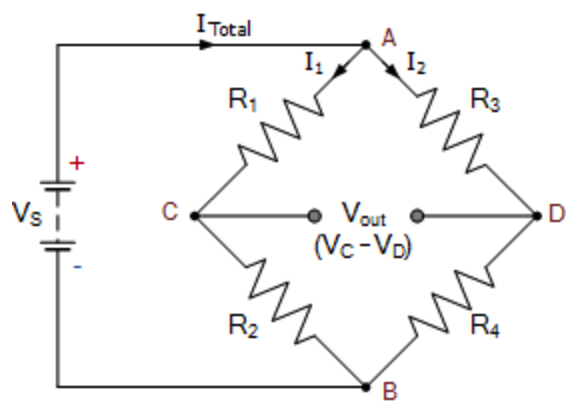
\includegraphics[width=0.5\textwidth]{Figurer/Snip20151207_63}
	\caption{Wheatstone bro}
\end{figure}

En Wheatstone bro er et kredsløb, der består af to serieforbindelser af to modstande, som sidder i parallelforbindelse. I mellem serieforbindelserne kan $V_{out}$ beregnes ud fra spændingen ved punkt C og punkt D.

\begin{equation}
	V_{out} = V_{C} - V_{D}
\end{equation} 

Hvis modstandene $R_{1}$ og $R_{3}$ samt $R_{2}$ og $R_{4}$ er ens, vil $V_{out}$ være lig med nul og broen vil være i balance, se Figur 3.4. 

\begin{figure}[H]
	\centering
	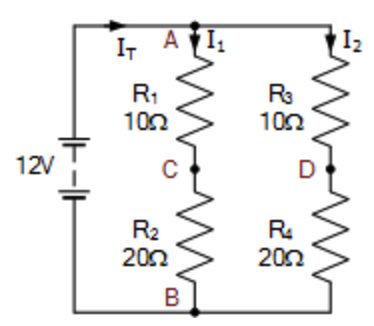
\includegraphics[width=0.5\textwidth]{Figurer/Snip20151207_64}
	\caption{Wheatstone bro i balance}
\end{figure}

Hvis modstandene $R_{1}$ og $R_{3}$ samt $R_{2}$ og $R_{4}$ er forskellige af hinanden, vil $V_{out}$ være forskellig fra nul og broen vil være i ubalance, se Figur 3.5. 

\begin{figure}[H]
	\centering
	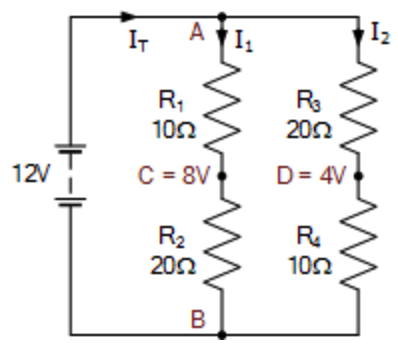
\includegraphics[width=0.5\textwidth]{Figurer/Snip20151207_65}
	\caption{Wheatstone bro i ubalance}
\end{figure}

Når trykændringerne påvirker membranen, vil de fire strain gauges ændre form og dermed ændre modstandsværdi. Dette skaber ubalance i Wheatestone broen, og spændingen ændrer sig i takt med dette. Spændingsændringen kan beregnes ud fra fomlen (3.5).


\begin{equation}
\centering
\frac{v_{0}}{v_{in}} = \frac{\Delta R}{R}
\end{equation}


\subsection{Dynamiske egenskaber}
Et væskefyldt kateter har inerti, friktion og elastiske egenskaber, der også kan betegnes som inertans, modstand og compliance (eftergivelighed). Disse egenskaber kan beskrives som elektriske komponenter i form af en induktor, resistor og kapacitor, se Figur 3.6.

\begin{figure}[H]
	\centering
	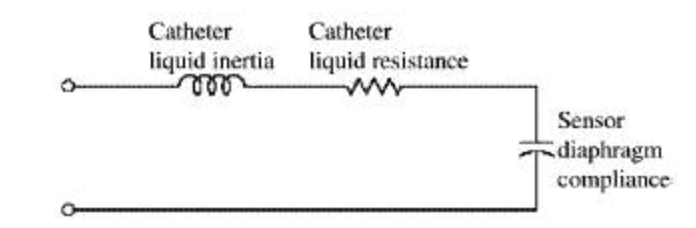
\includegraphics[width=1\textwidth]{Figurer/Snip20151207_58}
	\caption{Anden ordens lavpassystem}
\end{figure}

De forskellige egenskaber kan udtrykkes ved ligninger (3.6), (3.7) og (3.8). 

\begin{equation}
\centering
L = \frac{l\cdot p}{\pi\cdot r^2}
\end{equation}

\begin{equation}
\centering
R = \frac{8\cdot \mu\cdot l}{\pi\cdot r^4}
\end{equation}

\begin{equation}
C = \frac{\Delta V}{\Delta P} = \frac{1}{E_{d}}
\end{equation}

Figur 3.6 viser et anden ordens lavpassystem, der kan beskrives med følgende to overføringsfunktioner:

\begin{equation}
T(s) = \frac{K s}{s^2 + 2\cdot \zeta\cdot \omega_{0}\cdot s + \omega_{0}^2}
\end{equation}

\begin{equation}
T(s) = \frac{k}{s^2 + \frac{\omega_{0}}{Q} \cdot s + \omega_{0}^2}
\end{equation}

Ud fra disse overføringsfunktioner kan knækfrekvensen, $f_{0}$ og flowet, Q findes:

\begin{equation}
f_{0} = \frac{r}{2} \cdot \sqrt{\frac{1}{l\cdot p \cdot \pi}\cdot \frac{\Delta P}{\Delta V}}
\end{equation}

\begin{equation}
Q = \frac{r^3}{8 \cdot \mu} \cdot \sqrt{\frac{\rho \cdot \pi}{l}\cdot \frac{\Delta P}{\Delta V}}
\end{equation}
 \\
 
Figur 3.7 viser et bodeplot for amplitude og fasen for lavpasfilteret.

\begin{figure}[H]
	\centering
	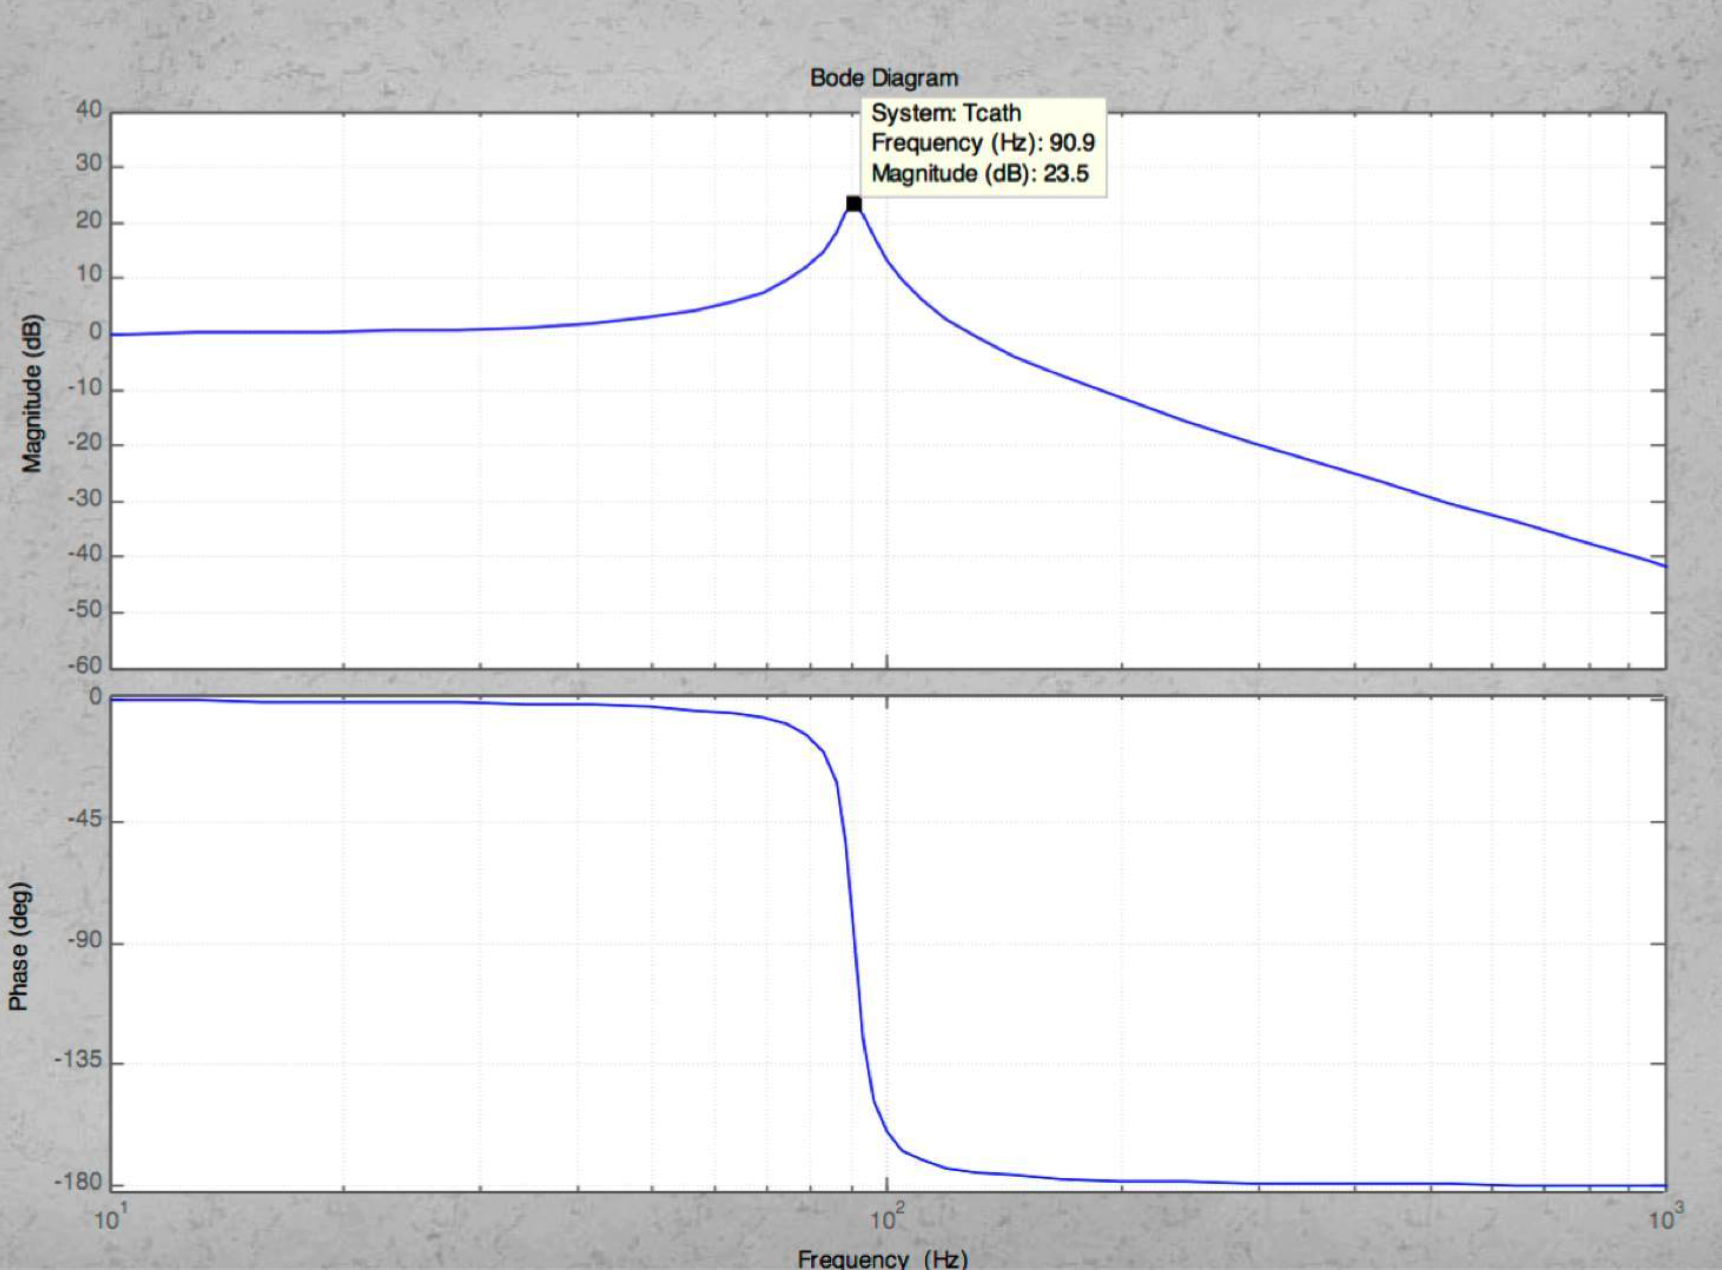
\includegraphics[width=0.8\textwidth]{Figurer/Snip20151207_61}
	\caption{Bodeplot}
\end{figure}

Det interessante er, at knækfrekvensen ligger ved 90 Hz. Dette betyder, at systemet medtager frekvenser op til de 90 Hz, hvilket er mere end, hvad systemet skal kunne klare ift. en blodtryksmåling, hvis frekvenser ikke kommer over 50 Hz.
\\\\ 

På figur 3.8 kan man se, hvorledes bobler i systemet påvirker systemets knækfrekvens og dermed dens båndbredde samt dæmpningsfaktoren.   

\begin{figure}[H]
	\centering
	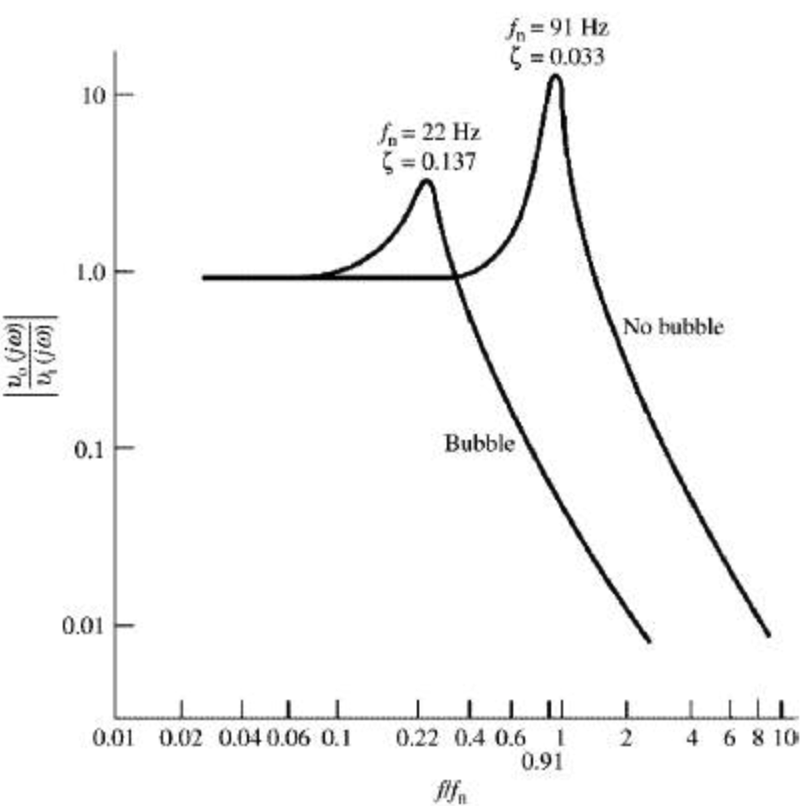
\includegraphics[width=0.5\textwidth]{Figurer/Snip20151207_62}
	\caption{Diagram over knækfrekvensen og dæmpningsfaktoren påvirket af bobler og uden}
\end{figure}

Hvis der er bobler tilstede i kateteret, bliver der samtidig tilført ekstra compliance. Dette medvirker til, at knækfrekvensen forekommer tidligere, hvilket betyder, at båndbredden bliver mindre. Som det ses i Figur 3.8 er knækfrekvensen mindre og dæmpningsfaktoren større, når der er bobler tilstede i kateteret.\\ 
En mindre knækfrekvens forårsager, at systemet kun lukker frekvenser fra 0 til 22 Hz igennem, hvilket ikke er tilstrækkeligt til at repræsentere en optimal blodtryksmåling. Dæmpningsfaktoren øges, når compliance stiger. Det vil sige, at jo større dæmpningsfaktor og compliance, jo mindre quality, jo større tab over system. Det ses ved ligningen for dæmpningsfaktoren:

\begin{equation}
\centering
\zeta = \frac{1}{2 \cdot Q}
\end{equation}

For at undgå bobler i væsken, kan man benytte føromtalte flushmekanisme, hvor man vha. trykposen kan erstatte luftbobler med natriumklorid.














